\documentclass[a4paper,english,12pt]{article}
% \usepackage{natbib}

%\usepackage[nosectionbib]{apacite}
\usepackage{babel}
\usepackage{footnote}
\usepackage{ucs} %sami letters
% \usepackage{amssymb} %mathematical
\usepackage[utf8x]{inputenc}
\usepackage[T1]{fontenc}
\usepackage{txfonts} %times roman
% \usepackage{a4wide}

\usepackage{color}
% \usepackage{hyperref}
\usepackage{graphicx}
\usepackage{covington}
\usepackage{url}
\usepackage[small,bf]{caption}
\usepackage{harvard}
\usepackage[right=2.5cm,left=2.5cm,top=2cm,bottom=2cm]{geometry}
% \usepackage{bibtexlogo}
\usepackage{setspace}
\usepackage{multirow}

\usepackage{fancyhdr}
\usepackage{linguex}


\begin{document}





\setcounter{secnumdepth}{3}
\setcounter{tocdepth}{3}
%\linespread{1.5}
\begin{spacing}{1.0}


\newcommand{\tx}{\mbox{t\hspace{-.35em}-}} % for S‡m

% \bibliographystyle{agsm} 


%Using meaning to disambiguate structure % through/with
\title{{\Large Workshop i Nordsamisk-lulesamisk maskinoversetting September 2009}} % \\[3ex]
%{\large such as Apertium and GramTrans \\[3ex]}}




\author{Trond Trosterud, Francis Tyers and Linda Wiechetek \\
		Universitetet i Tromsø and Universitat d'Alacant}
\date{23--24th September 2009}

\maketitle




%\thispagestyle{empty}
%\tableofcontents 
\thispagestyle{empty} %has to be after \maketitle

%\newpage
\setcounter{page}{1} %in order to start pagenumbering

\parindent = 0mm
\parskip = 12pt

%\begin{abstract} 
%preface, Acknowlegdments, or end of introduction or footnote to the title (latex)
%\end{abstract}


\section{Introduksjon}

\begin{itemize}
\item maskinoversetting i bilingual publisering (daglige aviser)
\item daglige aviser
\item skolebøker
\item flere tekster betyr også større etterspørsel
\end{itemize}

\textbf{Forventninger?}
 
\begin{itemize}
\item Hva forventer du av en oversetting?
\item Hva forventer du av maskinoversetting?
\end{itemize}


\section{Maskinoversetting}

Google, Babelfish, PROMT, Gramtrans


\begin{figure}
\centering
\scalebox{.5}[.5]{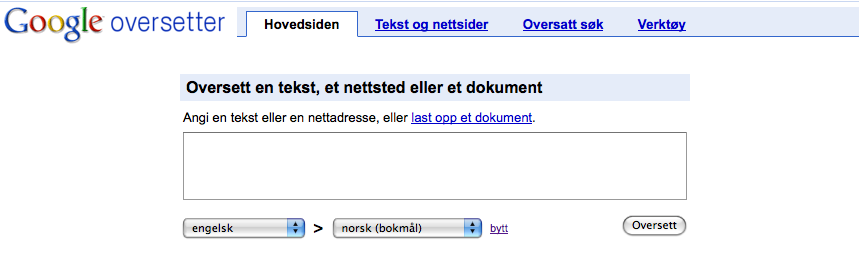
\includegraphics{google.png}} \\
  \caption{Google Translate: A popular online machine translation service}
\end{figure}
%\includegraphics<4>{PIC2}
%\includegraphics<6>{PIC3}
\begin{figure}
\centering
\scalebox{.5}[.5]{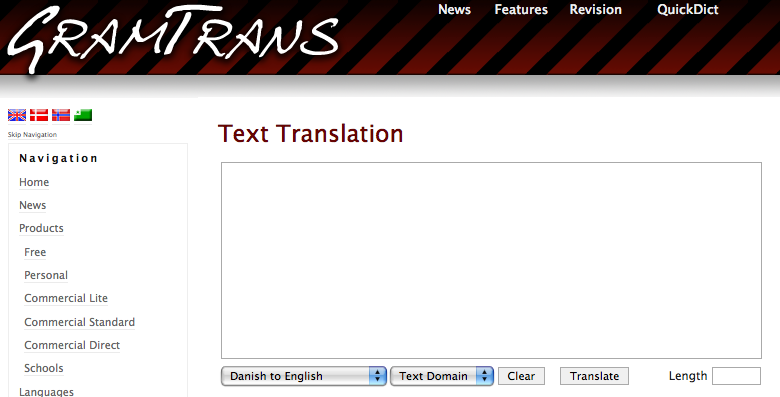
\includegraphics{gramtrans.png}}
  \caption{Gramtrans: Rule-based machine translation for the Scandinavian Germanic languages}
\end{figure}

\subsection{Eksempel på maskinoversetting}

\textbf{The Guardian 27.9.2009}
\begin{quote}
Last week, Iran said it was building a second uranium enrichment plant despite UN demands that it stops its development plans.
\end{quote}  


\textbf{Google en-nb}
\begin{quote}
Sist uke sa \textit{\textbf{subjekt?}} at Iran var det å bygge et \textbf{sekund} \textbf{anriking av uran anlegg} til tross for FNs krav om at den stopper sine utviklingsplaner.
\end{quote}  
% doesn't recognize the subject
% doesn't recognize the compound - anriking av uran anlegg

\textbf{Gramtrans en-nb}
\begin{quote}
Sist uke, sa Iran det holdt på å bygge et annen \textbf{uranberigelsesanlæg} tross \textbf{UN} krav \textbf{som} det stopper sine utviklingsplaner.
\end{quote}
% doesn't translate UN into FN

\textbf{Manuell oversetting}
\begin{quote}
Forrige uke sa Iran at de var i ferd med å bygge enda en urananrikingsfabrikk til tross for FNs krav om å stoppe utviklingsplanene.
\end{quote}


\textbf{Google nb-en} 
\begin{quote}
Last week, Iran said that they were about to build another \textbf{urananrikingsfabrikk} despite UN demands to halt development plans.
\end{quote}

\textbf{Gramtrans nb-en}
\begin{quote}
\textbf{Forrige} week Iran said that they were building still an \textbf{urananrichingsfabrikk} in spite of the UN's demand for stopping the development plans.
\end{quote}

 

\subsection{Hva er god oversetting?} 
\begin{itemize}
\item spesielt i forhold til skjønnlitterære tekster:
\item innhold vs. (kunstnerisk) budskap
\item ordrett vs. fri oversetting 
\item fremmedgjøring eller identifikasjon 
\end{itemize} 
 

\subsection{Det "samme" på forskjellige språk}
\begin{table}
\centering
\begin{tabular}{|c|c|}
\hline
\textbf{Språk} & \textbf{Navn} \\
\hline
Italiensk &  Paolino Paperino  \\
\hline
Kroatisk &  Paško Patak  \\
\hline
Kinesisk & Tánglăo Yā \\
\hline
Litauisk & Ančiukas Donaldas \\
\hline
Islandsk & Andrés Önd \\
\hline
Nordsamisk & Vulle Vuojaš \\
\hline
Engelsk & Donald Duck \\
\hline
\end{tabular}
\caption{Local adaptation: The name \emph{Donald Duck} translated into several languages.}
\end{table}
 

\subsection{Hva er god maskinoversetting?}

\textbf{Genesis 11,9 (New International Version (NIV))}
\begin{quote}
That is why it was called Babel because there the LORD confused the language of the whole world. From 
there the LORD scattered them over the face of the whole earth.
\end{quote}

\textbf{manuell ``oversetting''}
\begin{quote}
Derfor kalte de den Babel. For der forvirret Herren all verdens tungemål, og derfra spredte Herren dem ut over hele jorden.
-- \url{http://www.bibel.no}
\end{quote}

\textbf{Google}
\begin{quote}
Derfor ble det kalt Babel fordi det Herren forvirret språket i hele verden. Derfra spredte Herren dem over ansiktet til hele jorden.
\end{quote}
 
\textbf{Conclusions} 
\begin{itemize}
\item maskinoversetting oversetter ikke kulturelt ('ansiktet til hele jorden' passer ikke på norsk)
\item andere teksttyper er mer innholdsorientert: manual, avistekster
\end{itemize} 
 
\subsection{Uses of machine translation}


There are two main uses for machine translation, \emph{assimilation} and \emph{dissemination}:\\
~\\
\begin{table}
\centering
\begin{tabular}{l|l|l}
~  & Requirement & Not requirement\\
\hline
\multirow{3}{*}{Assimilation} & Understandability         & Syntactic \emph{correctness}\\
                              & \emph{Online} translation & Lexical \emph{correctness}\\
                              &                  & \\
\hline
\multirow{3}{*}{Dissemination} & Adequate syntactic transfer & Understandability \\
                               &  Predictable errors   & \emph{Online} translation \\
                               &  High accuracy (WER $\le$ 15\%)    & \\
\hline
\end{tabular}
\caption{Assimilation and dissemination: Features which are required and not required of both.}
\end{table}



\textbf{- Useful for assimilation, not dissemination:}\\


\emph{Erbyn heddiw mae Gaeleg yn dal yn iaith fyw yn y gogledd orllewin. }\\


By today a Scots Gaelic is tall in life language in the north west.\\


`Nowadays Scots Gaelic is still a living language in the north west.'\\ (WER = 43\%)\\

\textbf{- Useful for dissemination, not assimilation:}\\

\emph{Mae'r \textbf{mudiad} wedi derbyn canmoliaeth a beirniadaeth.}\\


The \textbf{migration} has received praise and criticism.\\

`The \textbf{organisation} has received praise and criticism.'\\ (WER = 14\%)\\


\subsection{God maskinoversetting:}
\begin{itemize}
  \item lik antall setninger
  \item nærmeste oversetting av ord
  \item syntaktisk struktur skal være så nært som mulig
  \item PoS skal være like
  \item innholdet skal ikke forandres
\end{itemize}
 


 
\subsection{What is machine translation?}

  \begin{centering}

    {\Large rule-based vs. statistical}

    (what we know vs. what we can infer)

  \end{centering}

 


 
\subsection{The {\tt apertium-sme-smj} system}

\begin{itemize}
  \item \underline{Prototype} system -- basically proof-of-concept
  \item Focussed heavily on reuse of existing resources -- testbed for 
    integrating Giellatekno work with Apertium
  \begin{itemize}
    \item Morphological transducers for North and Lule Sámi
    \item Constraint Grammar disambiguator
    \item Transfer lexicon (bilingual dictionary) built largely automatically
  \end{itemize}
  \item Still under development
\end{itemize}

 
\begin{figure}
\centering
\scalebox{.6}[.6]{\includegraphics{apertium-level2_simplified.pdf}}
\caption{A schematic of the Apertium translation pipeline.}
 \end{figure}


\section{Kontrastiv lingvistikk} 
\subsection{Emne}
\begin{itemize}
\item Something about contrastive linguistics  
\item Things we found out about Lule Sámi vs. North Sámi  
\item Orthography - how was the bilingual dictionary made  
\item dat/duot/dat vs.... 
\item Negation - tense marker in different elements  
\item SVO vs. SOV  
\item Case Loc vs. Ine/El  
\item Different PoS in some cases gullevaš vs. gullujiddje  
\item Why it can be interesting to work as a linguist -- being a discoverer  
\item Computational systems force you to be accurate -- when you need to be accurate you go into depth of linguistic questions
\end{itemize} 

\textbf{Hva skal vi med maskinoversetting?}
\begin{itemize}
\item maskinoversetting i bilingual publisering (daglige aviser)
\item daglige aviser
\item skolebøker
\item flere tekster betyr også større etterspørsel
\end{itemize}

\subsection{Hvordan brukes samisk Apertium?}

\begin{itemize}
\item Analysis
\item Disambiguation
\item Lexical transfer
\item Syntactic transfer
\item Generation
\end{itemize}

\textbf{Example}
\begin{quote}
Mun háliidan bargat "freelance" neavttárin go mu mielas oahppá olmmoš ollu eambbo go ferte bargat feara maid.
\end{quote}

%ja mun in vuos dieđe ahte álggán go Beaivváš Sámi Našunálateáhterii bistevaš virgái jus oaččun dákkár fálaldaga, čilge Ingá Márjá Sarre.
%Mån hálijdav barggat "*freelance" *neavttárin gå muv *mielas oahppá *olmmoš ållu ienebuv gå viertti barggat *feara aj ja mån iv vuostak diede ahte álgáv gå *Beaivváš Sámev *Našunálateáhterii *bistevaš *virgái jus oattjov dákkár *fálaldaga, tjielggi *Ingá *Márjá Sarrev.


\section{Lexicon}

\begin{figure}
\centering
\scalebox{.7}[.7]{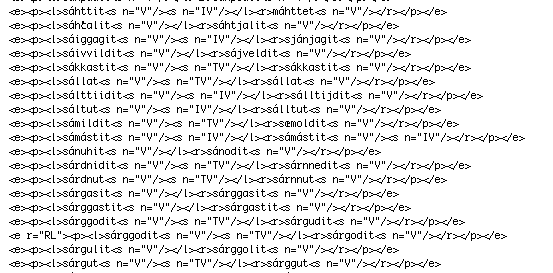
\includegraphics{bidix.png}}
  \caption{Bilingual dictionary: An example of some entries from the bilingual dictionary of the North--Lule Sámi system}
\end{figure}


\section{Lexical selection}
\begin{itemize}
\item "hui" - ihkeva, huj, alvos, riek...
\item "ráhkadit" - stiellit, tsieggit,dahkat, málestit
\item "váldit" - 
\item "sáhttit" - vissjat, máhttet, ...
\item "váldit gihtii" 
\item "diet" - dat, duot, ...
\end{itemize}


\section{Structural transfer} 
\begin{itemize}
  \item SOV rules
  \item (complexity of the objects, e.g. relative clauses)
  \item Case rules - different valency in North and Lule Sámi
  \item other structural rules??? (Ávvir)
\end{itemize}


\section{Evaluering}


\begin{itemize}
\item Hva forventer du av en oversetting?  
\item Hva forventer du av maskinoversetting?
\end{itemize}

\end{spacing}
\end{document}
